\section{Overview}

We introduce a physics-based technique to simulate strategic falling
and landing motions from a wide range of initial conditions. Our
control algorithm reduces joint stress due to landing impact and
allows the character to efficiently recover from the fall. The
character's motion is generated through a forward simulator and a
control algorithm that consists of an \emph{airborne phase} and a
\emph{landing phase}. These two phases are related by an appropriate
\emph{landing strategy}, which describes the body parts used for the
first contact with the ground, a desired landing pose, and an ideal
landing condition that describes the relation between landing
velocities and the angle of attack in successful landing motions. We
develop two most common types of landing strategies: hands-first and
feet-first, and introduce a sampling method to derive the ideal
landing condition for each strategy.

\begin{figure}
\center
  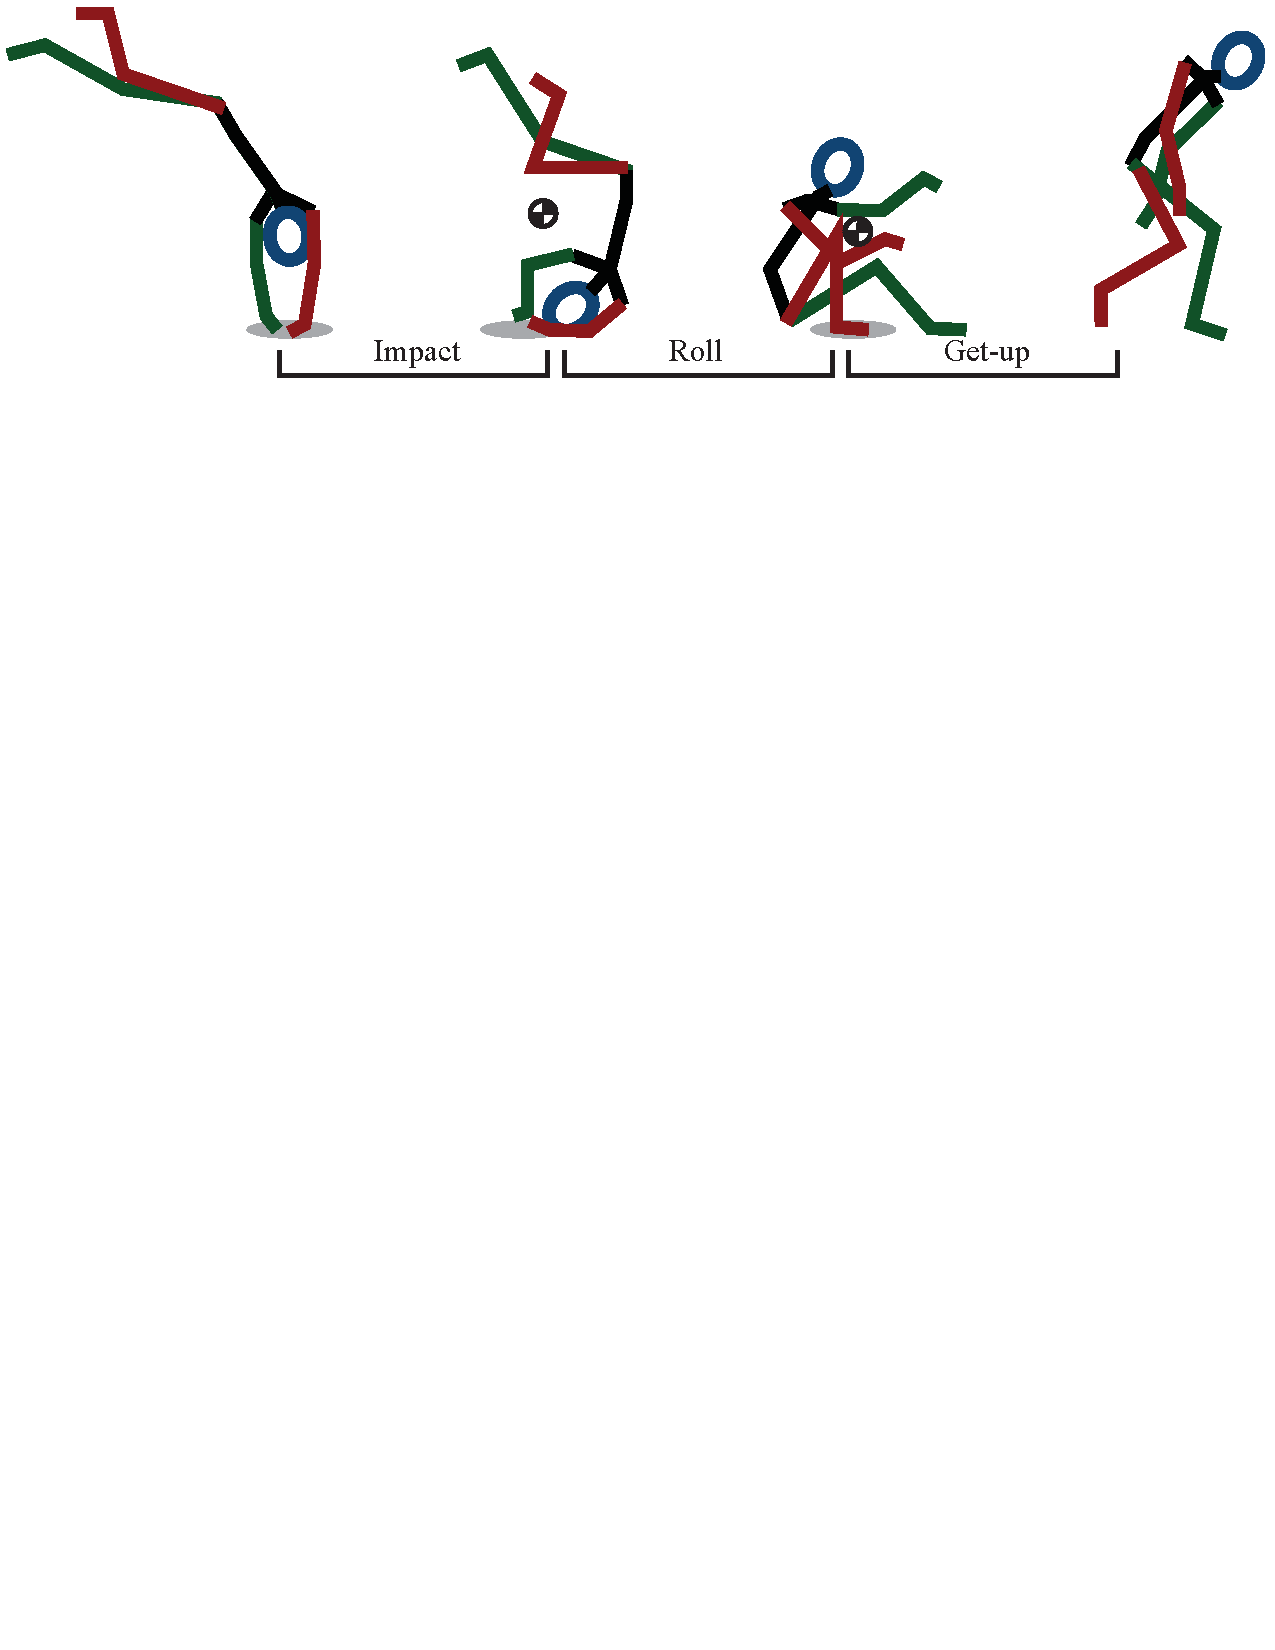
\includegraphics[width=4.2in]{images/landingPhase}
  \caption{Three stages in the landing phase.}
 \label{fig:landing_landingPhase}
\end{figure}

At the beginning of a fall, the character first decides on a landing
strategy. During the airborne phase, the character optimizes its
moment of inertia to achieve the ideal landing condition. The landing
phase is divided into three stages: impact, rolling, and getting-up
(Figure \ref{fig:landing_landingPhase}). The impact stage begins when the
character reaches the ground. 
%% During the impact stage, the character tries to control its linear 
%% and angular momentum while getting into a ready-to-roll pose. 
During the impact stage, the character leverages the friction forces 
from the ground to control linear and angular momentum. 
After the COM moves beyond the hand contact area,
the character switches to the rolling stage in which continuous change
of contact carries out. In preparation for standing up, the character
needs to maintain the rolling direction and plant its feet on the
ground. When the COM passes through the first foot, the character
starts to elevate the COM in order to compete the landing process in an
upright position.
